% !TEX TS-program = pdflatex
% !TEX encoding = UTF-8 Unicode

\documentclass{beamer}



\mode<presentation>
{
  \usetheme{Boadilla}
}


\usepackage[english]{babel}

\usepackage[utf8]{inputenc}
\usepackage{times}
\usepackage[T1]{fontenc}
\usepackage{graphicx}
\graphicspath{ {./photo/} }

\title[Strojno učenje] 
{Strojno učenje}

\author[Križnar Karel, Dobravec Blaž]
{Križnar Karel \and Dobravec Blaž}


\institute
{
  Praktična matematika\\
  Fakulteta za matematiko in fiziko
}
\date
{17.1.2019 / Seminar}

%fotografija
\pgfdeclareimage[height=1 cm]{university-logo}{photo/logo}
\logo{\pgfuseimage{university-logo}}





\beamerdefaultoverlayspecification{<+->}


\begin{document}

\begin{frame}
  \titlepage
\end{frame}





\section{Introduction}

\subsection[uvod]{Uvod}


%___________________________________________________
\begin{frame}
\frametitle[alignment=center]{Splošno} % ne delaaaaaa :(
  \begin{itemize}
  \item
    Kaj sploh je strojno učenje?
  \item
    Kje se strojno učenje uporablja?
  \item
    Umetna inteligenca = strojno učenje?
  \end{itemize}
\bigskip
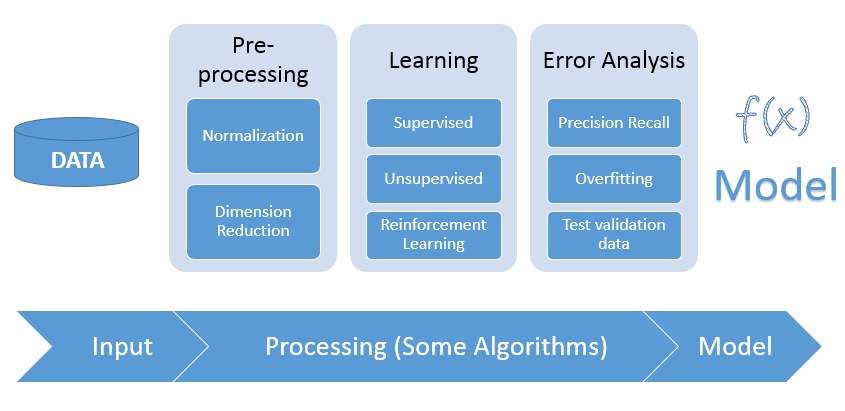
\includegraphics[scale = 0.3]{photo/ucenje_proces}
\end{frame}

\begin{frame}{Tipi strojnega učenja}
\bigskip
  Poznamo različne tipe strojnega učenja: \smallskip

  \begin{itemize}
  \item 
    \textbf{Nadzorovano učenje} $\rightarrow Algoritem $\texttt{ uči}  stroj na podlagi podanih parov vhodnih in željenih podatkov. Pri tem željene rezultate določa človek.
  \item 
     \textbf{Nenadzorovano učenje} $\rightarrow  Algoritem $\texttt{ razdeli} podatke v več skupin, ki imajo svoje značilnosti. Značilnosti algoritem izlušči iz vhodnih podatkov, brez pomoči človeka.
  \item 
     \textbf{Vzpodbujevalno učenje} $\rightarrow Algoritem $\texttt{ se priuči} vedenje oziroma optimizacijo vedenja na podlagi povratne informacije prek nagrajevanja oz. kaznovanja.
  \end{itemize}
\end{frame}

%___________________________________________________
\begin{frame}{Uporaba vsakega od tipov}
  \begin{itemize}
  \item
   Nadzorovano učenje
	\begin{itemize}
  	\item
   	  Napovedovanje vremena
  	\item
   	  \alert{Klasifikacija fotografij}
  	\item
   	  Ocenjevanje nevarnosti
	\end{itemize}
  \item
  Nenadzorovano učenje
    	\begin{itemize}
  	\item
   	  Medicinske raziskave
  	\item
   	  \alert{Ciljno in lokacijsko oglaševanje}
	\end{itemize}
  \item
   Vzpodbujevalno učenje
 	\begin{itemize}
  	\item
   	  Računalniške igre
  	\item
   	  \alert{Navigacija robotov}
  	\item
   	  Napovedovanje delnic
	\end{itemize}
  \end{itemize}
\end{frame}


\subsection{Prepoznavanje števil}

%___________________________________________________
\begin{frame}{Nevronska mreža}
\begin{itemize}
 \item
  Ideja strukture izhaja iz simuliranja delovanja nevronov v možganih
 \item
  Nevronska mreža je struktura, ki jo uporabljamo pri "učenju" računalnika
 \item
  Poznamo več različic nevronskih mrež
\end{itemize}
\begin{center}
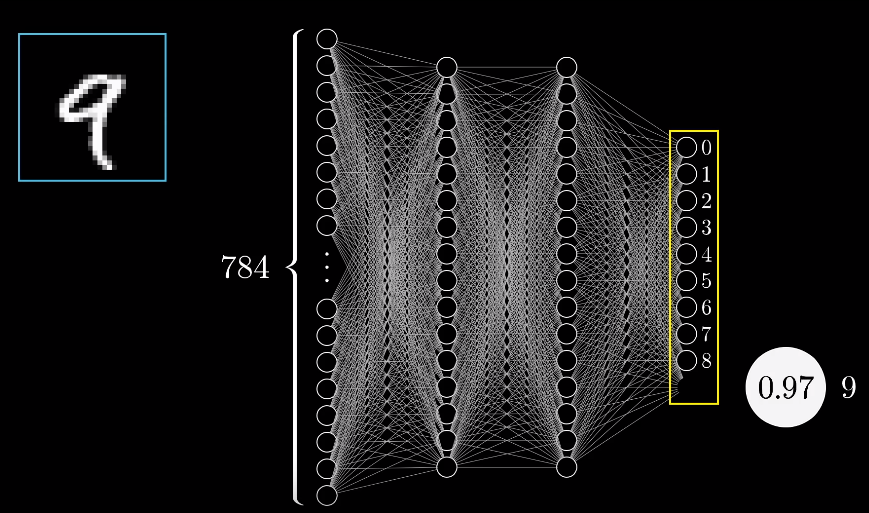
\includegraphics[scale = 0.3]{photo/foto3}
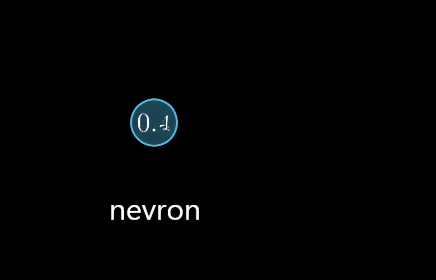
\includegraphics[scale = 0.3]{photo/nevron}
\end{center}
\begin{itemize}
\item
nevron je objekt, ki v sebi nosi številko, ki ji pravimo aktivacija nevrona
\end{itemize}
\end{frame}

%___________________________________________________
\begin{frame}{Prepoznavanje števil s pomočjo nevronske mreže}
\begin{itemize}
\item
Številka v nevronu pove kakšno barvo ima 0  $\rightarrow $ črn, 1  $\rightarrow $ bel
\item
V primeru bomo uporabljali $28*28$ pikslov veliko fotografijo
\end{itemize}
\begin{center}
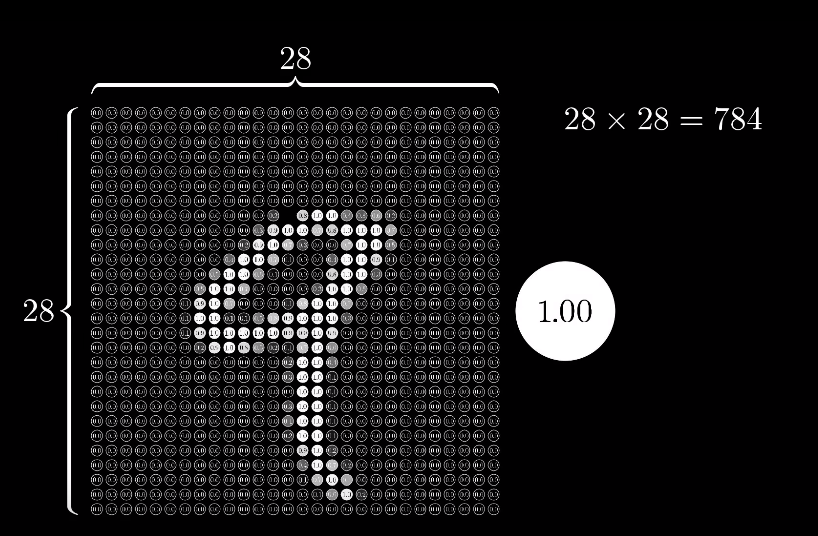
\includegraphics[scale = 0.45]{photo/foto2}
\end{center}
\end{frame}

%___________________________________________________
\begin{frame}{}
Aktivacija v zadnjem stolpcu $\rightarrow$ rezultat oz. kaj računalnik misli, da je na fotografiji
\begin{center}
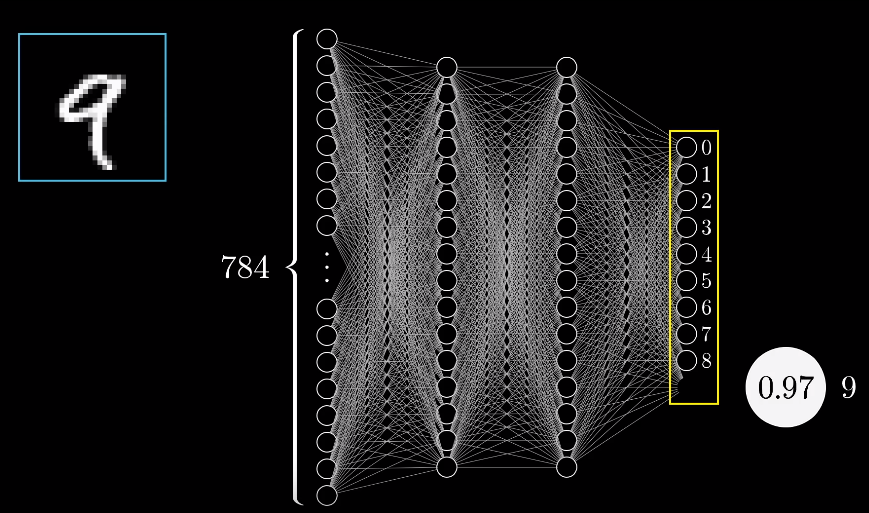
\includegraphics[scale = 0.55]{photo/foto3}
\end{center}
\end{frame}

%___________________________________________________
\begin{frame}{}
Vmesni stolpci $\rightarrow$ skriti nivoji \\
\smallskip
predstavljamo si jih lahko kot nivoje, ki pregledujejo del fotografije in ga rangirajo
\begin{center}
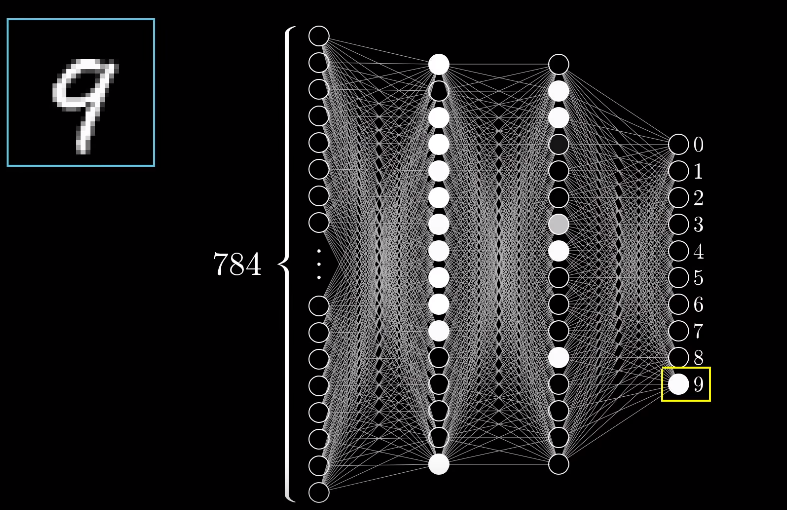
\includegraphics[scale = 0.55]{photo/foto4}
\end{center}
\end{frame}

%___________________________________________________
\begin{frame}{}
\begin{math}
a_1, a_2, a_3, ..., a_{n-1}, a_n
\end{math}
$ \rightarrow$ {to so aktivacije v sakemu od nevronom}

\begin{math}
w_1, w_2, w_3, ..., w_{n-1}, w_n
\end{math}
$ \rightarrow$ {to so uteži, na vsaki od povezav} $ \rightarrow$ te na začetku nastavimo poljubno

\begin{center}
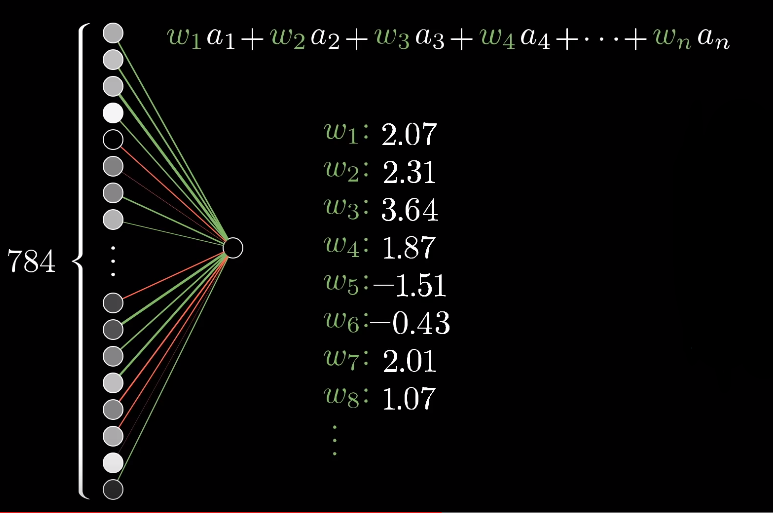
\includegraphics[scale = 0.5]{photo/foto6}
\end{center}
\end{frame}

%___________________________________________________
\begin{frame}{}
To število je poljubno. \\
\smallskip
Želimo si ga omejiti na interval $[0,1]$.\\
\smallskip
Uporabimo sigmoidno funkcijo.
\begin{center}
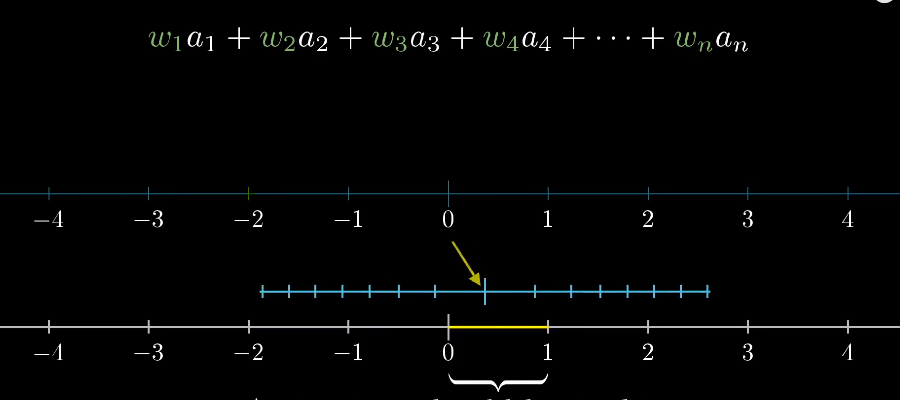
\includegraphics[scale = 0.55]{photo/foto7}
\end{center}
\end{frame}

%___________________________________________________
\begin{frame}{}
Vse skupaj lahko zapišemo v matrični obliki. \\
\smallskip
Dodamo še takoimenovani "bias" oziroma korekcijo. \\
\bigskip

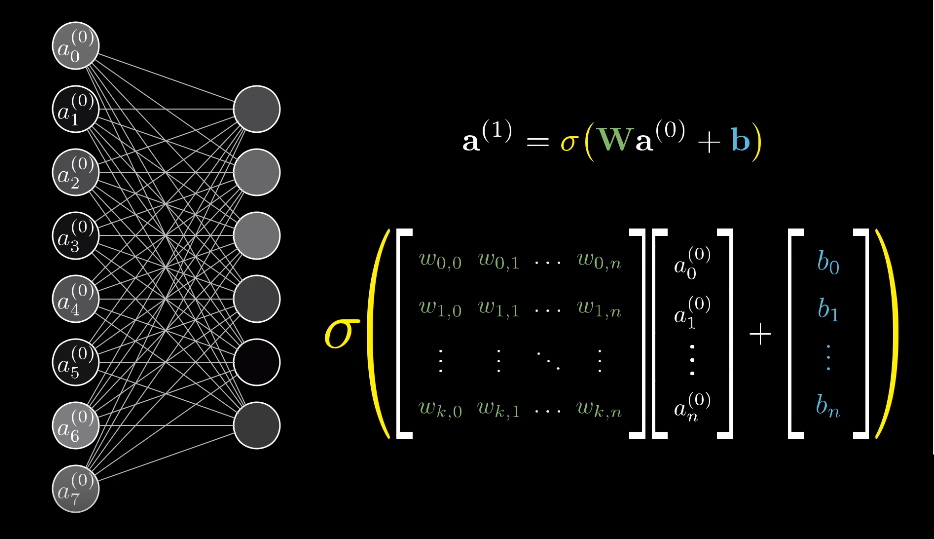
\includegraphics[scale = 0.27]{photo/foto8}
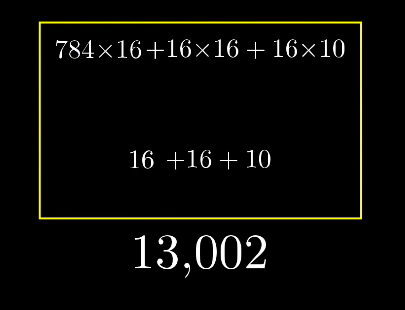
\includegraphics[scale = 0.3]{photo/foto9} \\

\bigskip
Imamo natanko 13.002 možnih parametrov, ki jih lahko spreminjamo.
\end{frame}

%___________________________________________________
\begin{frame}{}
Definirajmo cenovno funkcijo, ki bo povedala, kako dobro je računalnik prepoznal število.\\
\smallskip
Preverimo vse testne primere (za katere vemo željeni rezultat) in izračunamo kvadrate razlike ter vse skupaj seštejemo.
\smallskip
\begin{center}
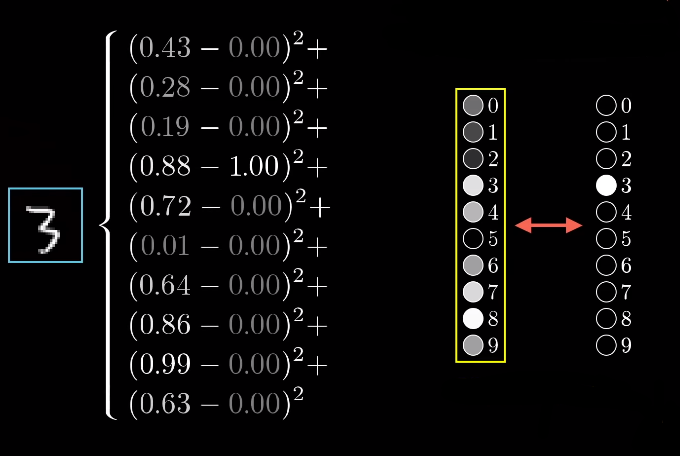
\includegraphics[scale = 0.35]{photo/2foto3} \\
\end{center}
\smallskip
Če bo računalnik z zagotovostjo povedal katero število bo to bo cenovna funkcija blizu 0. \\
\smallskip
Cenovna funkcija je torej funkcija, ki dobi 13.002 parametra in vrne eno število.
\end{frame}
 
%___________________________________________________
\begin{frame}{}
Predstava funkcijo z eno spremenljivko.\\
\smallskip
\begin{center}
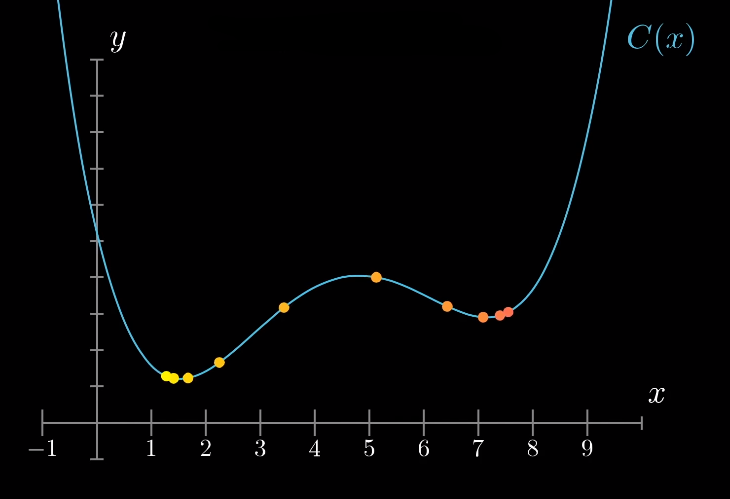
\includegraphics[scale = 0.3]{photo/2foto1} \\
\end{center}

Želimo minimizirati cenovno funkcijo $\leftarrow$ spreminjamo parametre. \\

Računanje gradienta $\rightarrow$ Izračunamo (parcialne) odvode. \\
Majhen premik v smeri gradienta $\rightarrow$ ponovno računanje gradienta
\end{frame}

%___________________________________________________
\begin{frame}{}
Iz vseh uteži in korekcij ustvarimo vektor .\\
\smallskip
Vektor, ki pa ga dobimo s pomočjo gradienta pa prištejemo prvotnemu vektorju. \\

\begin{center}
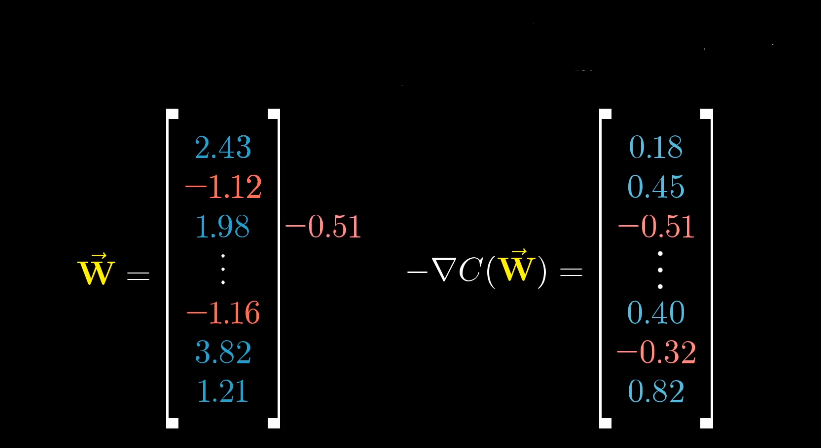
\includegraphics[scale = 0.35]{photo/2foto4} \\
\end{center}

S tem spremenimo vse te parametre $\rightarrow$ Temu algoritmu pravimo vzvratno razširjanje oz. Backpropagation.
\end{frame}



\section*{Summary}

\begin{frame}{Summary}

  % Keep the summary *very short*.
  \begin{itemize}
  \item
    The \alert{first main message} of your talk in one or two lines.
  \item
    The \alert{second main message} of your talk in one or two lines.
  \item
    Perhaps a \alert{third message}, but not more than that.
  \end{itemize}
  
  % The following outlook is optional.
  \vskip0pt plus.5fill
  \begin{itemize}
  \item
    Outlook
    \begin{itemize}
    \item
      Something you haven't solved.
    \item
      Something else you haven't solved.
    \end{itemize}
  \end{itemize}
\end{frame}


\end{document}


